\documentclass[border=10pt, linewidth]{standalone} % 修改了这里，增加了 border=10pt
\usepackage{tikz}
\usetikzlibrary{shapes, arrows.meta, positioning, calc, shadows, fit, backgrounds}
\usepackage{xcolor}

% 定义颜色
\definecolor{sedarRed}{RGB}{220, 53, 69}
\definecolor{morphGreen}{RGB}{25, 135, 84}
\definecolor{codeBg}{RGB}{248, 249, 250}

\begin{document}

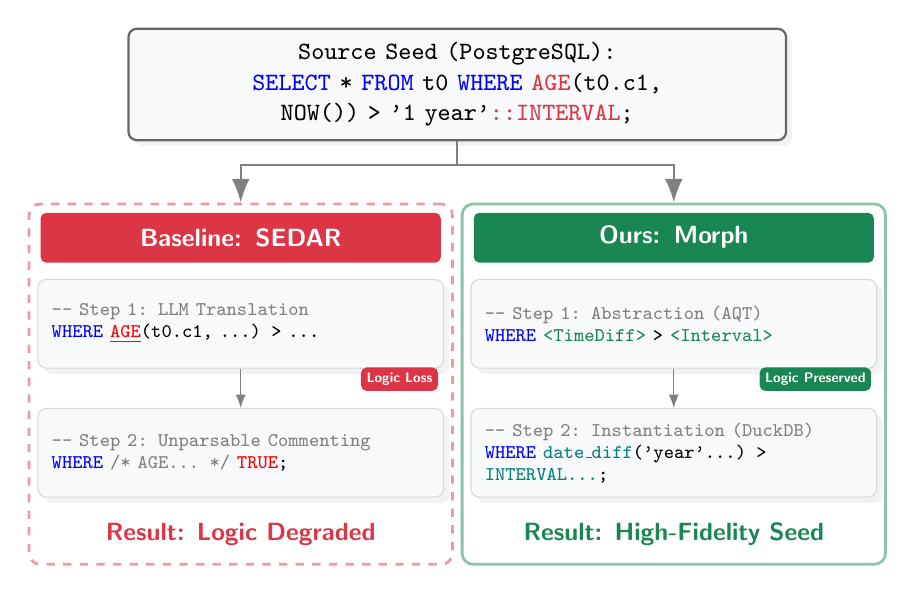
\begin{tikzpicture}[
    node distance=0.5cm, 
    font=\small,
    box/.style={
        rectangle, 
        draw=gray!30, 
        fill=codeBg, 
        rounded corners=3pt, 
        inner sep=5pt,
        align=left,
        font=\ttfamily\scriptsize, 
        drop shadow={opacity=0.1},
        minimum height=3.2em % 统一步骤框高度
    },
    header/.style={
        font=\sffamily\bfseries\small,
        text=white,
        align=center,
        minimum height=1.8em,
        rounded corners=2pt,
        inner sep=4pt
    },
    labelTag/.style={
        font=\sffamily\tiny\bfseries,
        inner sep=2pt,
        rounded corners=2pt,
        text=white,
        yshift=0.6em,
        xshift=-0.2em
    },
    resultText/.style={
        font=\sffamily\bfseries\small,
        align=center,
        minimum height=1.5em % 统一结果文字框高度
    }
]

% -----------------------------------------------------------
% 1. Input Source Query
% -----------------------------------------------------------
\node[box, align=center, text width=8cm, draw=black!60, line width=0.8pt, font=\ttfamily\small, minimum height=0pt] (input) {
    \textbf{Source Seed (PostgreSQL):}\\
    \textcolor{blue}{SELECT} * \textcolor{blue}{FROM} t0 \textcolor{blue}{WHERE} \textcolor{sedarRed}{AGE}(t0.c1, NOW()) > '1 year'\textcolor{sedarRed}{::INTERVAL};
};

% 定位参照点
\node[below=0.7cm of input.south, xshift=-2.75cm] (sedarHeaderPos) {};
\node[below=0.7cm of input.south, xshift=2.75cm] (morphHeaderPos) {};

% ===========================================================
% LEFT COLUMN: SEDAR
% ===========================================================
\node[box, below=0.8cm of sedarHeaderPos, text width=4.8cm] (sedarStep1) {
    \textcolor{gray}{-- Step 1: LLM Translation}\\
    \textcolor{blue}{WHERE} \textcolor{red}{\underline{AGE}}(t0.c1, ...) > ...
};
\node[labelTag, fill=sedarRed, anchor=south east] at (sedarStep1.north east) {Hallucination};

\node[box, below=0.5 cm of sedarStep1, text width=4.8cm] (sedarStep2) {
    \textcolor{gray}{-- Step 2: Unparsable Commenting}\\
    \textcolor{blue}{WHERE} \textcolor{gray}{/* AGE... */} \textcolor{red}{\textbf{TRUE}};
};
\node[labelTag, fill=sedarRed, anchor=south east] at (sedarStep2.north east) {Logic Loss};

\node[resultText, text=sedarRed, below=0.2cm of sedarStep2] (sedarResult) {Result: Logic Degraded};

\draw[-{Latex}, gray] (sedarStep1) -- (sedarStep2);
\node[header, fill=sedarRed, above=0.2cm of sedarStep1, text width=4.8cm] (sedarTitle) {Baseline: SEDAR};

\begin{scope}[on background layer]
    \node[fit=(sedarTitle)(sedarStep1)(sedarStep2)(sedarResult), 
          draw=sedarRed!50, dashed, rounded corners, inner sep=3pt, line width=1pt] (sedarFrame) {};
\end{scope}

% ===========================================================
% RIGHT COLUMN: Morph
% ===========================================================
\node[box, below=0.8cm of morphHeaderPos, text width=4.8cm] (morphStep1) {
    \textcolor{gray}{-- Step 1: Abstraction (AQT)}\\
    \textcolor{blue}{WHERE} \textcolor{morphGreen}{<TimeDiff>} > \textcolor{morphGreen}{<Interval>}
};
\node[labelTag, fill=morphGreen, anchor=south east] at (morphStep1.north east) {Intent Decoupled};

\node[box, below=0.5cm of morphStep1, text width=4.8cm] (morphStep2) {
    \textcolor{gray}{-- Step 2: Instantiation (DuckDB)}\\
    \textcolor{blue}{WHERE} \textcolor{teal}{date\_diff}('year'...) > \textcolor{teal}{INTERVAL...};
};
\node[labelTag, fill=morphGreen, anchor=south east] at (morphStep2.north east) {Logic Preserved};

\node[resultText, text=morphGreen, below=0.2cm of morphStep2] (morphResult) {Result: High-Fidelity Seed};

\draw[-{Latex}, gray] (morphStep1) -- (morphStep2);
\node[header, fill=morphGreen, above=0.2cm of morphStep1, text width=4.8cm] (morphTitle) {\textbf{Ours: Morph}};

\begin{scope}[on background layer]
    \node[fit=(morphTitle)(morphStep1)(morphStep2)(morphResult), 
          draw=morphGreen!50, rounded corners, inner sep=3pt, line width=1pt] (morphFrame) {};
\end{scope}

% -----------------------------------------------------------
% Main Connecting Arrows
% -----------------------------------------------------------
\draw[-{Latex[length=3mm]}, thick, gray] (input.south) -- ++(0,-0.3) -| (sedarFrame.north);
\draw[-{Latex[length=3mm]}, thick, gray] (input.south) -- ++(0,-0.3) -| (morphFrame.north);

% Marks (只保留 Morph 的打勾)
\node[right=0.05cm of morphResult, text=morphGreen, font=\large\bfseries] {$\checkmark$};

\end{tikzpicture}
\end{document}